\documentclass[times, twoside, watermark]{artigo}
\usepackage{blindtext}
\usepackage[utf8]{inputenc}
\citebrackets[]
\usepackage{indentfirst}
\renewcommand\refname{}
% \documentclass[article, 12pt, oneside, a4paper, twocolumn]{abntex2}
% \usepackage[left=3cm,top=3cm,right=2cm,bottom=2cm]{geometry}
% \usepackage[alf, abnt-etal-list=0, abnt-etal-cite=3]{abntex2cite}
% \usepackage{authblk}
% \usepackage{amsmath}
% \usepackage{amsfonts}
% \usepackage{amssymb}
% \usepackage{graphicx}
% \usepackage{verbatim}
% \usepackage{titlesec}

\begin{document}

% -------------------------------Titulo---------------------------------------------

\title{\Large {Desenvolvimento de firmware robusto e multiplataforma}}

\author[1]{Jonathan Gonzaga}
\author[2]{Orientador}

\affil[1]{Graduando em Engenharia de Computação, UNISAL São José - Campinas,
\href{mailto:jonathan.s.gonzaga@gmail.com}{jonathan.s.gonzaga@gmail.com}}
\affil[2]{Professor do UNISAL São José - Campinas,
\href{mailto:orientador@sj.unisal.br}{orientador@sj.unisal.br}}

\maketitle

% -------------------------------Resumo-Abstract-------------------------------------

\noindent\begin{abstract}
\textit{Resumo -} \normalfont{\textit{Este artigo apresenta técnicas e ferramentas 
para o desenvolvimento de firmware robusto e multiplataforma, com o intuito de 
minimizar bugs, permitir a implementação de testes unitários e incentivar o estudo de 
conceitos de Engenharia de software aplicados a sistemas embarcados.}}
\end {abstract}

\noindent\begin{keywords}
\textit{\textbf{Palavras-chave: }}\normalfont{\textit{sitemas embarcados, firmware, 
TDD, testes unitários}}
\end{keywords}

\noindent\begin{abstract}
\textit{Abstract - } \normalfont{\textit{This article presents techniques and tools 
for robust and multiplatform firmware development, in order to minimize bugs, allow 
the implementation of unit tests and encourage the study of software engineering 
concepts applied to embedded systems.}}
\end {abstract}
\noindent\begin{keywords}
\textit{\textbf{Keywords: }}\normalfont{\textit{embedded systems, firmware, TDD, unit 
tests}}
\end{keywords}
%\hfill\

% -------------------------------INTRODUÇÃO-----------------------------------------

\section{INTRODUÇÃO }

Com o avanço da eletrônica e da computação, a miniaturização de circuitos integrados
e a redução de custos de fabricação, surgiram na indústria diversos dispositivos
eletrônicos com poder de processamento. 
A maioria desses dispositivos conta com processadores, memórias e periféricos
integrados, de forma que seu \textit{software} é destinado e \textit{embarcado} 
em uma aplicação específica. Sistemas dessa natureza são conhecidos como
\textit{sistemas embarcados}.

Produtos como eletrodomésticos, eletrônicos em geral, equipamentos médicos,
equipamentos de telecomunicações, ferramentas eletrônicas, sistemas de controle 
e automação e sistemas de tempo real em veículos são ou possuem sistemas embarcados
em sua concepção.

Devido ao alto nível de criticidade de alguns sistemas embarcados, é esperado que o
\textit{software} executado neles seja altamente confiável e com o mínimo de
\textit{bugs} possível. 
A realidade da indústria de eletrônicos mostra que essa afirmação nem sempre é 
verdadeira.

Erros e falhas de \textit{software} são um problema em diversas áreas da tecnologia. 
Desde vulnerabilidades que facilitam a ação de \textit{hackers} em redes sociais,
falhas em \textit{smartphones} que causam travamento do sistema operacional a
inconsistências no acionamento de sistemas de freios que causam acidentes em
veículos. Esse último caso é ainda mais grave, pois o sistema lida diretamente com
vidas humanas. 

Especialistas em desenvolvimento de \textit{firmware} e \textit{software} embarcado, 
como Jack Ganssle, James W. Grenning e Jacob Beningo, dedicaram-se a criar 
literatura de qualidade, escrevendo livros e artigos com técnicas e 
metodologias de desenvolvimento de \textit{software}. 
Alguns títulos relevantes são: \textit{Test-Driven development for Embedded C}
\cite{tddembeddedc}, 
\textit{The Art of Designing Embedded Systems}\cite{ganssle2008art} e
\textit{Reusable Firmware Development}\cite{beningo2017reusable}. 
A partir dessas obras muito se tem discutido sobre como criar sistemas mais seguros, 
com menor probabilidade de erros e menos suscetíveis a má utilização por parte do 
usuário.

No processo de desenvolvimento de \textit{software}, o custo de uma alteração no 
código tende a ficar maior conforme  as etapas do desenvolvimento avançam, por isso 
o custo de um \textit{bug} encontrado em campo após o produto ser lançado, é muito 
maior que o custo do mesmo sendo encontrado ainda na fase de 
desenvolvimento\cite{firmwarecost}.
Esse cenário por si só já mostra a necessidade de se detectar problemas nas fases 
iniciais do projeto.

\textit{Software} para sistemas embarcados muitas vezes é difícil de ser testado e 
validado, extremamente dependente da plataforma de \textit{hardware target}, e 
tende a demonstrar problemas de integração com outras
partes do sistema após a inserção de novas funcionalidades. 
Devido a limitação de recursos e a extrema dependência do \textit{hardware}, testes 
automatizados não são realizados, o que acaba prejudicando a qualidade do código.

Metodologias e conceitos como \textit{TDD (Test-Driven development)}, pirâmide de 
testes e \textit{SOLID}, são historicamente e erroneamente atribuídos apenas
aos \textit{softwares} de "alto nível", como \textit{web} ou 
\textit{mobile} por exemplo, afastando os desenvolvedores de \textit{software} 
embarcado desses conceitos e da utilização de abstrações mais inteligentes. 

Com essas dificuldades em mente, percebe-se a necessidade de se estimular as boas 
práticas de desenvolvimento de \textit{software} embarcado, a utilização de testes 
automatizados e independentes do \textit{hardware}, e o estudo de conceitos de 
engenharia de \textit{software} que auxiliem na
redução de \textit{bugs} e consequentemente, redução de custos do projeto e aumento 
da qualidade do código gerado. \hfill\\



% ----------------------REFERENCIAL TEÓRICO-----------------------------------

\section{REFERENCIAL TEÓRICO}

\subsection{Firmware}\hfill\\

\textit{Firmware} é um tipo específico de \textit{software} executado diretamente
num circuito integrado (ou \textit{chip}). 
Não necessita de outros programas para ser executado (como sistemas operacionais),
além de servir a um propósito único. 
Em outras palavras, é o \textit{software} executado em um sistema
embarcado\cite{ganssle2004firmware}.

Devido a limitações de tamanho e recursos desse tipo de sistema, 
o \textit{firmware} precisa manipular o \textit{hardware} diretamente e toda a sua
arquitetura costuma ser voltada a eventos do mundo externo.

Diferente de sistemas computacionais mais complexos e com alto nível de abstração,
onde geralmente o \textit{kernel} do sistema operacional é modularizado e abstrai
o acesso a dispositivos de \textit{hardware}\cite{tanenbaum2015modern},
num sistema embarcado o \textit{firmware} é responsável pela gerência dos recursos 
e eventos de \textit{hardware} (interrupções e exceções do processador) e também
pelo código da aplicação (regras de negócio, interface com usuário e demais 
especificidades).

Muitas vezes ele faz parte de um sistema computacional maior,
por exemplo, computadores \textit{desktop} possuem circuitos integrados para 
aplicações específicas, como a \textit{BIOS} (\textit{Basic Input/Output System}),
que trata-se de um mecanismo responsável pela inicialização dos
componentes de \textit{hardware} do computador. \cite{terzicbasic}

Algumas literaturas não fazem distinção entres os termos \textit{firmware} e 
\textit{software embarcado}, sendo ambos utilizados como sinônimos. Por uma
questão de organização, será realizada uma distinção entre
esses termos: \textit{firmware} é o \textit{software} executado num circuito 
integrado comumente escrito em linguagem \textit{C, C++}, ou mesmo \textit{Assembly}. 
Já o \textit{software embarcado} possui características de alta abstração, 
sendo uma aplicação (um processo rodando num sistema operacional, 
geralmente baseado em \textit{GNU/Linux})\cite{simmonds2015mastering} porém executado 
em dispositivos de propósito específico (como roteadores e terminais de 
autoatendimento). 
Pode ser escrito em linguagens de programação como \textit{C, C++, Rust, Go, Python} 
entre outras.

Em um sistema embarcado executando um \textit{firmware}, o cérebro por trás de todo o 
processamento é um componente chamado \textit{microcontrolador}.

\subsection{Microcontroladores}\hfill\\

Microcontroladores são processadores de pequeno porte contendo \textit{CPU}, 
memórias (\textit{RAM} e \textit{FLASH}) e demais
recursos atrelados no mesmo encapsulamento ou \textit{SoC (System on Chip)}.
Esses recursos são denominados periféricos, e são inclusos no \textit{chip} 
com o intuito de tornar possível o interfaceamento entre a \textit{CPU} 
e o mundo externo, permitir a comunicação com outros dispositivos e 
aquisitar dados para posterior processamento através dos pinos físicos do componente.

Os recursos mais comuns são as interfaces de comunicação 
serial (\textit{USART, I2C, SPI}), conversores analógico-digital e digital-analógico 
(\textit{ADC} e \textit{DAC}), temporizadores/contadores (\textit{TIMERS}) e 
interface de pinos (\textit{GPIO}).

Com tamanho e custo reduzidos em comparação ao microprocessadores,
os microcontroladores tornam-se economicamente viáveis, além da
escolha óbvia, para controlar digitalmente dispositivos e 
processos\cite{gridling2007introduction}.


\subsection{Linguagem de programação - \textit{C}}\hfill\\

\textit{C} é uma linguagem de programação procedural de propósito geral que 
suporta programação estruturada, escopo de variável lexical e recursão, com um 
sistema de tipo estático. Por design, \textit{C} fornece construções que mapeiam de 
forma eficiente para instruções de máquina típicas. Dispõe de compiladores para a 
maioria das arquiteturas de computador e sistemas operacionais 
existentes.\cite{ritchie1993development}

Devido a essas características, vem  sendo utilizada em aplicações previamente 
codificados em linguagem \textit{assembly}. 
Algumas dessas aplicações são: sistemas operacionais, compiladores,
\textit{drivers} de dispositivos, bibliotecas com acesso a \textit{hardware} e 
sistemas embarcados.

Leva esse nome por ser sucessora da linguagem de programação \textit{B}.
Foi desenvolvida no \textit{Bell Labs} por Dennis Ritchie entre 1972 e 1973 para 
construir utilitários rodando em \textit{Unix}. 
Em 1989 foi padronizada pelo \textit{ANSI} (\textit{ANSI C}) e pela 
\textit{International Organization for Standardization (ISO)}.
\cite{ritchie1993development}

\subsection{Testes de \textit{software}}\hfill\\

Testes de \textit{software} são procedimentos pelos quais o código fonte de um
\textit{software} é submetido afim de validar seu comportamento mediante
os requisitos pelos quais foi projetado.

Existem diversos tipos de testes de \textit{software}, cada um responsável por 
testar partes e situações diferentes. A chamada \textit{Pirâmide de testes}
\cite{contan2018test} foi concebida com o intuito de seguimentar os testes em três 
grandes níveis:

\begin{itemize}
\item \textit{Testes end-to-end} - simulam a aplicação final
\item \textit{Testes de integração} - testa a integração entre testes de unidade
\item \textit{Testes unitários} - testes de unidade, verificam a menor unidade de 
código testável
\end{itemize}

Apenas o último nível, os testes unitários, serão abordados nesse documento.

\subsection{Testes unitários}\hfill\\

Testes unitários são a base dos testes de \textit{software}. Na \textit{Pirâmide de 
testes} encontram-se no nível mais baixo, o que indica que são 
o tipo mais barato e fácil de implementar\cite{contan2018test}, 
fazendo com que sejam os mais numerosos em relação aos demais tipos de teste.

Como seu nome sugere, são testes de \textit{unidade}, onde é possível testar a 
menor unidade testável do código (sejam funções, classes ou módulos).

\subsection{\textit{TDD - Test-Driven development}}\hfill\\

\textit{Test-Driven development} (ou \textit{Desenvolvimento orientado a testes}) é 
uma técnica incremental de construção de \textit{software}. 
Nessa técnica, nenhum código de produção é escrito sem que primeiro seja escrito um 
teste unitário que falhe na primeira execução. 

Ao contrário da prática comum de desenvolvimento de \textit{software}, onde primeiro 
é desenvolvido o código de produção e só depois os testes, no TDD
o desenvolvedor expressa o comportamento desejado do código em um teste. 
O teste é executado e falha. Só então ele escreve o código de produção, fazendo o 
teste passar.
A automação de testes é a chave para o \textit{TDD}. Os testes são pequenos e 
automatizados.
A cada nova funcionalidade implementada, novos testes unitários são escritos, 
seguidos imediatamente por um código de produção que satisfaça aqueles testes. 

Conforme o código de produção cresce, também crescem em conjunto os testes unitários, 
que são ativos tão valiosos quanto o próprio código de produção. 
A cada mudança de código, o conjunto de testes é executado, verificando a 
funcionalidade da nova implementação, mas também a compatibilidade com o código já 
existente\cite{tddembeddedc}.

Um esquema simplificado do \textit{TDD} é apresentado na Figura \ref{fig:tdd}:\hfill\

\begin{figure}[H]
    \centering
    \caption{Esquema simplificado do TDD}
    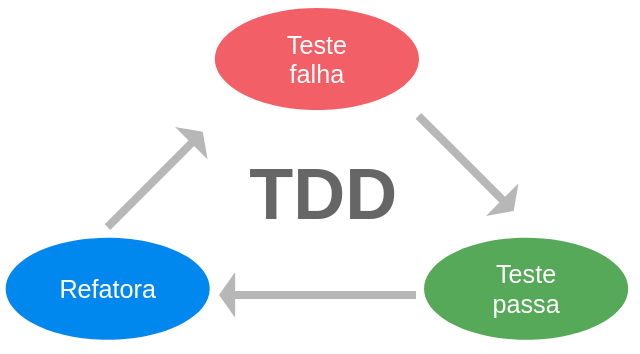
\includegraphics[width=0.95\linewidth]{images/tdd.png}
    \caption*{\newline\textbf{Fonte:} acervo do autor}
    \label{fig:tdd}
\end{figure}

Três grande etapas são necessárias: \textit{Teste falha}, \textit{Teste passa}
e \textit{Refatora}. Na primeira, são escritos apenas os testes unitários, com base 
nos requisitos do projeto, porém sem nenhum código de produção ainda, o que 
obviamente fará com que os testes falhem após a execução.

Logo após, são escritos apenas os trechos de código necessários para que aqueles 
testes passem e nada mais.

Na última etapa, o código passará pelo processo de \textit{refatoração}, onde serão 
eliminados possíveis erros, duplicidade, e será formatado de acordo com o padrão 
requisitado.


\subsection{\textit{Framework} de testes - \textit{Unity}}\hfill\\

\textit{Unity} é um \textit{framework} de testes escrito em linguagem C, pensado 
principalmente para \textit{software} em sistemas embarcados.

Trabalha com o conceito de \textit{asserts}, que nada mais são que formas de se 
garantir e verificar parâmetros (entrada) e resultados (saída) de funções no código 
fonte.\cite{unity}


\subsection{Ferramenta de dublês de testes - \textit{CMock}}\hfill\\

\textit{CMock} é uma ferramenta de dublês de testes, usada para simular o 
comportamento de funções que possuam dependência externa (\textit{hardware} ou 
bibliotecas externas).

Trabalha com os conceitos de \textit{mocks} e \textit{stubs}, 
que nada mais são que funções \textit{fake}, criadas com o intuito de emular o 
comportamento (entradas e saídas) de componentes do código que tenham alguma 
dependência.\cite{cmock}

\subsection{\textit{Build system - Ceedling}}\hfill\\

\textit{Ceedling} é um \textit{build system} (sistema de construção de 
\textit{software}) para projetos escritos em linguagem C.
É uma espécie de extensão do sistema de construção \textit{Rake (make-ish)} do 
\textit{Ruby}.
O \textit{Ceedling} é voltado principalmente para o 
\textit{Desenvolvimento Orientado a Testes (TDD)} em linguagem C e reune o 
\textit{framework} de testes \textit{Unity}, a ferramenta de dublês de testes 
\textit{CMock} e a ferramenta de manipulação de exceções \textit{CException} - três 
outros projetos de código aberto que auxiliam na dinâmica de testes 
automatizados\cite{gomes2016uttos}.

\subsection{Sistema operacional de tempo real - \textit{FreeRTOS}}\hfill\\

\textit{FreeRTOS} é um \textit{kernel} de tempo real, 
ou um sistema operacional de tempo real (\textit{Real-Time Operating System}) 
para dispositivos embarcados. Foi desenvolvido para ser pequeno, simples e portável. 
Seu \textit{kernel} é composto por apenas 3 arquivos em linguagem C. 
O \textit{FreeRTOS} permite a fácil implementação de multitarefa preemptiva 
ou não preemptiva com diversos níveis de prioridade de 
tarefas\cite{zhu2016understanding}.\hfill\\

\subsection{\textit{Build system - GNU Make}}\hfill\\

\textit{GNU Make} é um \textit{build system} (sistema de construção de 
\textit{software}) que controla a geração de executáveis de um \textit{software}
a partir dos arquivos de código fonte.

A ferramenta \textit{Make} recebe as instruções de como construir o programa a partir 
de um arquivo chamado \textit{makefile}, que lista cada um dos arquivos de código 
fonte e os comandos para transformá-los em executáveis. 

Ao escrever um programa, deve-se escrever um \textit{makefile} para ele, de modo 
que seja possível usar o \textit{Make} para construção e execução do mesmo.
\cite{gnumake}

\subsection{Compilador - \textit{GCC}}\hfill\\

O \textit{GNU Compiler Collection (GCC)} é um compilador de otimização produzido pelo 
\textit{Projeto GNU} que oferece suporte a várias linguagens de programação, 
arquiteturas de \textit{hardware} e sistemas operacionais. 

A \textit{Free Software Foundation (FSF)} distribui o \textit{GCC} como 
\textit{software livre} sob a licença \textit{GNU General Public License (GNU GPL)}.
O \textit{GCC} é um componente chave da cadeia de ferramentas \textit{GNU} e o 
compilador padrão para a maioria dos projetos relacionados ao \textit{GNU} e ao 
\textit{kernel Linux}.\cite{gcc}


\subsection{Editor de textos - \textit{Visual Studio Code}}\hfill\\

O \textit{Visual Studio Code} é um editor de código-fonte \textit{freeware} feito 
pela \textit{Microsoft} para \textit{Windows}, \textit{Linux} e \textit{macOS}. Os 
recursos incluem suporte para depuração, destaque de sintaxe, autocompletar de código 
inteligente, \textit{snippets}, refatoração de código e \textit{Git}
incluso.\cite{vscode}


% ----------------------METODOLOGIA-----------------------------------
\section{METODOLOGIA}

\subsection{MATERIAIS E MÉTODOS}\hfill\\
%Reseta o contador de subsection
% \setcounter{section}{-1}\stepcounter{section}

Serão utilizadas as seguintes ferramentas de \textit{software} na execução do projeto:

\begin{itemize}
\item \textit{FreeRTOS} - sistema operacional de tempo real
\item \textit{GNU make} - \textit{Build system} para compilação do código de produção
\item \textit{GCC(x86)} e \textit{GCC(arm)}- compiladores para ambas arquiteturas
\item \textit{VS Code} - editor de textos
\item \textit{Ceedling} - \textit{Build system} para compilação e execução dos testes
\item \textit{Unity} - \textit{framework} de testes
\item \textit{Cmock} - ferramenta de dublê de testes
\end{itemize}

A metodologia utilizada para o desenvolvimento do projeto segue a técnica de 
\textit{TDD} descrita anteriormente.

Nas três etapas (\textit{Teste falha}, \textit{Teste passa}
e \textit{Refatora}) serão utilizadas ferramentas e mecanismos de \textit{software} 
para auxílio na implementação dos testes, execução e automatização de processos \hfill\

% ----------------------DESENVOLVIMENTO-----------------------------------

\subsection{DESENVOLVIMENTO}\hfill\\

%Reseta o contador de subsections
% \setcounter{section}{-1}\stepcounter{section}
O processo de desenvolvimento do projeto seguiu o padrão especificado anteriormente,
juntamente com algumas regras e boas práticas:

\begin{itemize}
\item \textit{Clean Code} (Código limpo) - o código precisa ser de fácil 
entendimento\cite{martin2009clean}
\item \textit{KISS (Keep it simple stupid)} - as soluções implementadas precisam ser 
simples\cite{martin2018clean}
\item \textit{SOLID principles} - seguir os padrões do \textit{SOLID}
\cite{martin2002agile}
\item \textit{Boy Scout Principle} (Regra do escoteiro) - \textit{"Deixe o campo mais 
limpo do que quando o encontrou"} - Sempre deixe o código melhor do antes de você 
trabalhar nele\cite{martin2009clean}
\item \textit{Refactoring} (Refatoração) - o código precisa ser refatorado e 
aprimorado constatemente\cite{martin2009clean}
\end{itemize}

\subsubsection{Arquitetura de \textit{software} do sistema}\hfill\\
Os componentes de \textit{software} separados por nível de abstração estão ilustrados 
na Figura \ref{fig:arch2}.\hfill\\

\begin{figure}[H]
    \centering
    \caption{Arquitetura de software do projeto}
    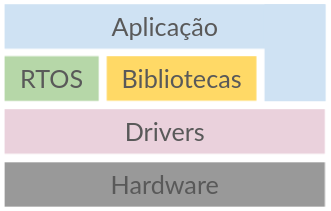
\includegraphics[width=0.9\linewidth]{images/arch2.png}
    \caption*{\newline\textbf{Fonte:} acervo do autor}
    \label{fig:arch2}
\end{figure}

A camada de \textit{Aplicação} faz uso dos \textit{Drivers} para controle dos 
periféricos de \textit{hardware}, utiliza o \textit{RTOS} para criar e gerenciar
\textit{threads} e recursos compartilhados por elas e as \textit{Bibliotecas}
fornecem alguma funcionalidade extra como \textit{file system} (sistema de arquivos)
ou cálculo de \textit{PID (Proporcional - Integral -Derivativo)} por exemplo.

\subsubsection{Camadas de abstração - \textit{drivers}, Bibliotecas e \textit{RTOS}}\hfill\\

Um dos pilares do desenvolvimento de \textit{software} multiplataforma é a abstração.
Utilizar interfaces bem definidas a partir de \textit{header files} (arquivos de 
extensão \textit{.h}), variando apenas a implementação dessas interfaces nos 
\textit{source files} (arquivos de extensão \textit{.c}).

Para se escrever código portável é extremamente necessário a não dependência de 
\textit{Drivers}, \textit{RTOS - (Real Time Operating Systems)} e demais bibliotecas

A abordagem consiste em criar camadas de abstração que acessem essas camadas, como 
pode ser visto na Figura \ref{fig:arch-abs}:\hfill\\

\begin{figure}[H]
    \centering
    \caption{Arquitetura de software com abstrações}
    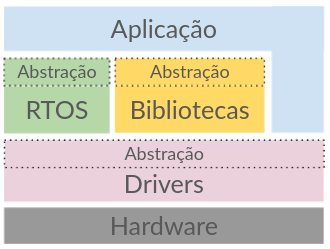
\includegraphics[width=0.9\linewidth]{images/arch-abs.png}
    \caption*{\newline\textbf{Fonte:} acervo do autor}
    \label{fig:arch-abs}
\end{figure}


Essas camadas são apenas funções que encapsulam as funções dos módulos originais, 
fazendo com que o código da \textit{Aplicação} nunca realize uma chamada de função 
diretamente a esses componentes, mas sim as suas abstrações.

Imaginemos um exemplo de módulo dependente de \textit{hardware},
responsável pelo acionamento de pinos de um microcontrolador. O módulo de 
\textit{GPIO - General Purpose Input Output}. Esse módulo é um \textit{driver} e está 
localizado na camada de mesmo nome:

\begin{lstlisting}[language=C, caption=Interface do módulo de GPIO - gpio.h]
#ifndef __GPIO_H__
#define __GPIO_H__

void gpio_config(int port, int pin);
int gpio_read(int port, int pin);
void gpio_write(int port, int pin, int level);

#endif
\end{lstlisting}


\begin{lstlisting}[language=C, caption=Implementação do módulo de GPIO - gpio.c]
#include "gpio.h"

void gpio_config(int port, int pin)
{
    GPIO.port.CFG |= pin;
}

int gpio_read(int port, int pin)
{
    return GPIO.port.RD.pin;
}

void gpio_write(int port, int pin, int level)
{
    GPIO.port.WR.pin = level;
}
\end{lstlisting}

O módulo contém funções que dependem do \textit{hardware}, porém as mesmas não 
devem ser chamadas diretamente pela aplicação, mas sim por uma abstração:

\begin{lstlisting}[language=C, caption=Interface pública do módulo - gpio\_iface.h]
#ifndef __GPIO_IFACE_H__
#define __GPIO_IFACE_H__

#include "gpio.h"

void gpio_iface_config(int port, int pin);
int gpio_iface_read(int port, int pin);
void gpio_iface_write(int port, int pin,
                      int level);
#endif
\end{lstlisting}


\begin{lstlisting}[language=C, caption=Implementação da abstração para acesso ao 
módulo de GPIO - gpio\_iface.c]
#include "gpio_iface.h"

void gpio_iface_config(int port, int pin)
{
    // Chama a funcao do modulo original
    gpio_config(port, pin);
}

int gpio_iface_read(int port, int pin)
{
    // Chama a funcao do modulo original
    return gpio_read(port, pin);
}

void gpio_iface_write(int port, int pin, int level)
{
    // Chama a funcao do modulo original
    gpio_write(port, pin, level);
}
\end{lstlisting}


A abstração do módulo, chamada de de \textit{gpio\_iface.c e gpio\_iface.h} 
(\textit{iface} é uma abreviação para \textit{interface}) abstrai o 
acesso, permitindo que seja feita a utilização de dublês de testes (\textit{mocks, 
fakes e stubs}), visando a implementação de testes unitários.

A aplicação final faz uso apenas do módulo de abstração:

\begin{lstlisting}[language=C, caption=Camada de aplicação - main.c]
#include <stdio.h>
// Camada de aplicacao nao inclui o modulo
// diretamente, mas sim sua abstracao
#include "gpio_iface.h"

int main(void)
{
    gpio_iface_config(PORT_C, PIN_13);
    
    // Loop infinito
    while (1) {
        // Classico exemplo de pisca led
        gpio_iface_write(PORT_C, PIN_13, 1);
        delay_ms(500);
        gpio_iface_write(PORT_C, PIN_13, 0);
        delay_ms(500);
    }
    return 0;
}
\end{lstlisting}


\subsubsection{Implementando testes unitários}\hfill\\

A implementação de testes unitários exige a utilização de um \textit{framework}
de testes. Foi utilizado o \textit{Unity}, ferramenta já contida no \textit{Ceedling}. 
Usando os comandos do próprio \textit{build system} para a criação
do projeto, temos a seguinte linha de comando:

\begin{lstlisting}[language=bash, caption=Criando um projeto com o \textit{Ceedling}]
$ ceedling new projeto-exemplo
\end{lstlisting}

Uma estrutura de diretórios semelhante a mostrada abaixo é criada:\hfill\

\begin{forest}
      for tree={
        font=\ttfamily,
        grow'=0,
        child anchor=west,
        parent anchor=south,
        anchor=west,
        calign=first,
        inner xsep=7pt,
        edge path={
          \noexpand\path [draw, \forestoption{edge}]
          (!u.south west) +(7.5pt,0) |- (.child anchor) pic {folder} \forestoption{edge label};
        },
        % style for your file node 
        file/.style={edge path={\noexpand\path [draw, \forestoption{edge}]
          (!u.south west) +(7.5pt,0) |- (.child anchor) \forestoption{edge label};},
          inner xsep=2pt,font=\small\ttfamily
                     },
        before typesetting nodes={
          if n=1
            {insert before={[,phantom]}}
            {}
        },
        fit=band,
        before computing xy={l=15pt},
      }
[projeto-exemplo
  [build]
  [src]
  [test]
  [project.yml, file]
]
\end{forest}

\begin{itemize}
\item \textit{build} - contém os artefatos de \textit{software}, arquivos temporários 
e executáveis
\item \textit{src} - contém o código fonte da aplicação
\item \textit{test} - contém o código fonte dos testes
\item \textit{project.yml} - contém a configuração relativa ao projeto
\end{itemize}

Para criar o primeiro módulo, usamos \textit{ceedling module:create} passando o nome 
do módulo como argumento:

\begin{lstlisting}[language=bash, caption=Criando um módulo com o \textit{Ceedling}]
$ ceedling module:create[gpio]
\end{lstlisting}


A ferramenta criará arquivos \textit{source} e \textit{header} em \textit{src} e um 
arquivo de testes em \textit{test}:

%\dirtree{%
%.1 projeto-exemplo.
%.2 build.
%.3 gpio.c.
%.3 gpio.h.
%.2 src.
%.2 test.
%.3 test\_gpio.c.
%.2 project.yml.
%}

\begin{forest}
      for tree={
        font=\ttfamily,
        grow'=0,
        child anchor=west,
        parent anchor=south,
        anchor=west,
        calign=first,
        inner xsep=7pt,
        edge path={
          \noexpand\path [draw, \forestoption{edge}]
          (!u.south west) +(7.5pt,0) |- (.child anchor) pic {folder} \forestoption{edge label};
        },
        % style for your file node 
        file/.style={edge path={\noexpand\path [draw, \forestoption{edge}]
          (!u.south west) +(7.5pt,0) |- (.child anchor) \forestoption{edge label};},
          inner xsep=2pt,font=\small\ttfamily
                     },
        before typesetting nodes={
          if n=1
            {insert before={[,phantom]}}
            {}
        },
        fit=band,
        before computing xy={l=15pt},
      }
[projeto-exemplo
  [build]
  [src
    [gpio.c, file]
    [gpio.h, file]
  ]
  [test
    [test\_gpio.c, file]
  ]
  [project.yml, file]
]
\end{forest}


No arquivo de testes, são criadas as funções, \textit{setUp()} e 
\textit{tearDown()} e adicionado o \textit{header file unity.h}:

\begin{lstlisting}[language=C, caption=Arquivo de testes inicial]
#include "unity.h"
#include "gpio.h"

void setUp(void)
{
}

void tearDown(void)
{
}

void test_gpio_NeedToImplement(void)
{
    TEST_IGNORE_MESSAGE(
        "Need to Implement gpio");
}
\end{lstlisting}

Utilizando as abstrações demonstradas anteriormente, os primeiros testes podem ser 
implementados:

\begin{lstlisting}[language=C, caption=Arquivo de testes com um teste simples]
#include "unity.h"
#include "gpio.h"

void setUp(void)
{
}

void tearDown(void)
{
}

void test_gpio(void)
{
    TEST_ASSERT_EQUAL(0, 
        gpio_iface_read(PORT_C, PIN_13));
}
\end{lstlisting}

\subsubsection{Utilizando dublês de teste}\hfill\\

Dublês de teste são utilizados nos casos em que há dependência de algum componente 
externo e o módulo precisa ser testado. O \textit{driver} de \textit{GPIO} é um 
exemplo de dependência de \textit{hardware}, nesse caso, é interessante o uso 
de dublês de teste. A ferramenta responsável pela geração desses dublês é o 
\textit{Cmock}.

\begin{lstlisting}[language=C, caption=Arquivo de testes com mock]
#include "unity.h"
#include "mock_gpio.h"

void setUp(void)
{
}

void tearDown(void)
{
}

// Callback utilizada ser chamada pelo Cmock
int gpio_iface_read_callback(int cmock_num_calls)
{
    return 1;
}

void test_gpio(void)
{
    // Registrando a callback
    gpio_iface_read_StubWithCallback(
        gpio_iface_read_callback);
        
    TEST_ASSERT_EQUAL(0, 
        gpio_iface_read(PORT_C, PIN_13));
}
\end{lstlisting}


No código anterior uma função de \textit{callback} é definida e registrada no 
\textit{Cmock}, de modo que toda vez que a função original for chamada,
\textit{gpio\_iface\_read()}, a ferramenta redireciona a chamada para 
\textit{gpio\_iface\_read\_callback()}. Para isso é necessário apenas incluir 
o \textit{header file} com o prefixo \textit{mock\_}: \textit{mock\_gpio.h}.

O argumento \textit{cmock\_num\_calls} na \textit{callback} é uma obrigatoriedade
da ferramenta, para que haja o controle do número de chamadas realizadas a 
\textit{callback}.


\begin{lstlisting}[language=bash, caption=Rodando o primeiro teste com \textit{Ceedling}]
$ ceedling test:all
Test 'test_gpio.c'
------------------------------
Generating include list for gpio.h...
Creating mock for gpio...
Generating runner for test_gpio.c...
Compiling test_gpio_runner.c...
Compiling test_gpio.c...
Compiling mock_gpio.c...
Compiling unity.c...
Compiling gpio.c...
Compiling cmock.c...
Linking gpio.out...
Running gpio.out...

--------------------
OVERALL TEST SUMMARY
--------------------
TESTED:  1
PASSED:  1
FAILED:  0
IGNORED: 0
\end{lstlisting}

\subsubsection{Dual-targeting: compilando para duas arquiteturas}\hfill\\

O processo de \textit{Dual-targeting} só é possível quando se consegue independência
entre os módulos de software.




% ----------------------CONCLUSÃO-----------------------------------

\section{CONCLUSÃO}\hfill\\
Conclui-se que 


% \section{REFERÊNCIAS}
\bibliography{artigo}

\end{document}
